%
\documentclass[11pt, a4paper, uplatex]{jsarticle}
\usepackage{graphicx}
\usepackage{amsmath,amssymb}
\usepackage{theorem}
\usepackage{bm}
\usepackage{ascmac}
\usepackage{subfigure}
\usepackage{multicol}
\usepackage{setspace}
\usepackage{mediabb}
\usepackage{float}
\usepackage{latexsym}
\usepackage{url}
\usepackage{cite}
\usepackage{layout}

\makeatletters
%
\def\@thesis{Master Thesis}
\def\@gakui{2014年度 修士論文}
\def\title#1{\def\@title{#1}}
\def\daimoku#1{\def\@daimoku{#1}}
\def\id#1{\def\@id{#1}}
\def\department#1{\def\@department{#1}}
\def\shozoku#1{\def\@shozoku{#1}}
\def\author#1{\def\@author{#1}}
\def\chosha#1{\def\@chosha{#1}}
\def\chosha#1{\def\@chosha{#1}}
\def\submission#1{\def\@submission{#1}}
%
\def\@maketitle{
\begin{center}
{\huge \@thesis \par}
\vspace{10mm}
{\huge \@gakui \par}
\vspace{10mm}
{\LARGE\bf \@daimoku \par}% 論文のタイトル部分
\vspace{10mm}
{\Large \@title \par} %
\vspace{10mm}
{\Large \@submission \par} %
\vspace{20mm}
{\Large \@shozoku \par}
{\Large 学籍番号 \@id \par} % 学籍番号部分
\vspace{10mm}
{\LARGE \@chosha \par}

\vspace{20mm}
{\Large \@department \par}
\vspace{10mm}
{\LARGE \@author}
\end{center}
%\par\vskip 1.5em
\clearpage
}
%
\renewcommand{\theequation}{\arabic{section}.\arabic{equation}}
\@addtoreset{equation}{section}
%
\theorembodyfont{\normalfont}
\newtheorem{theorem}{定理}
%\newtheorem{definition}[theorem]{定義}
\newenvironment{proof}[1][\proofname]{\par
%\newenvironment{Proof}[1][\Proofname]{\par
  \normalfont
  \topsep6\p@\@plus6\p@ \trivlist
  \item[\hskip\labelsep{\bfseries #1}\@addpunct{\bfseries.}]\ignorespaces
}{%
  \endtrivlist
}
\newcommand{\proofname}{証明}
%%%%%%%%%%%%%%%%%%%%%%%%
\newcommand{\subcaption}[1]{
\begin{center}
\begin{minipage}{0.8 \hsize}
\centering \small \ \ #1
\end{minipage}
\end{center}
}
%%%%%%%%%%%%%%%%%%%%%%%%
\makeatother
%
\daimoku{Multipath TCPを用いたデータセンターネットワークの改善}
\title{Improving the datacenter network with multipath TCP}
\date{\today}
\shozoku{東京大学大学院 \\ 工学系研究科 電気系工学専攻}
\department{The University of Tokyo \\ Graduate School of Engineering,
Department of Electrical Engineering and Information Systems}
\id{37-136482}
\chosha{藤居 翔吾}
\author{Fujii Shogo}
\submission{平成26年 2月5日 提出}
%
\begin{document}
%
\maketitle
\tableofcontents
\clearpage

\listoftables
\clearpage

\listoffigures
\clearpage


\section{序論}

\subsection{研究背景}
今日の一般家庭のインターネット接続環境がギガビット級の速度に達しようとしている中, 多様な端末がインターネットに接続できるようになり,
大量かつ多種多様なデータの取得が可能となった.
特にトラフィックデータ量の増加傾向は顕著で, 18$\sim$24ヶ月単位で総データ容量が2倍になるという予測がされている~\cite{IBM_rep}.
またFacebookでは, 300ペタバイト以上のデータ量を保有しており, 1日あたりに1ペタバイトのデータを解析している~\cite{presto}.
このように近年では, ビッグデータの活用が着目され, 例えばウェブ検索エンジン, SNS(Social Networking
Service)などのデータセンターを用いたクラウド型サービスにおいて, リアルタイムに近いレスポンスを返すような場面で使われ始めている.
そのようなクラウドサービスには近年, より高いユーザーエクスペリエンスが要求されており,
Amazonでは100[ms]の遅延により売り上げが1\%下がる, といった報告~\cite{amazon}があるように,
例えばeコマースサイトでの商品購入や,
インターネット広告のコンバージョンのようなユーザの意思決定へのレスポンス遅延の影響は深刻な問題である~\cite{customer_impact}.
そのため, 大規模データをより高速に処理することが求められており, データセンターではサーバ運用台数が増加の一途を辿っている.
そうした中で, 可用性, 計算性能, 低コストの三つの要件がデータセンターの抱える課題となっている~\cite{requirement}.
特に計算性能について, 大量の計算機資源から最大限の性能を引き出すためには,
従来の仕組みではデータセンター内トラフィックに対して一部の資源にトラフィックが集中する問題に対応できないため,
計算機資源を有効活用するための研究が盛んに行われている\cite{mapreduce, fattree,
dctcp, improving, detail, p_fab, synchro}.
そのようなスケーラビリティ拡大には, ネットワークトポロジー, アプリケーション, プロトコルに対する三つのアプローチがある.

ネットワークトポロジーを改良するアプローチでは, 従来の単純な階層構造では,
データセンター内で発生するトラフィックに対して帯域が最大限割り当てられない~\cite{fattree}.
そのため,
近年ではそのようなトラフィックに対してスイッチを多段に構成することで帯域を有効利用するトポロジーが提案されており,
マルチパス環境を実現している~\cite{fattree}.

大量データの処理速度を改良するアプローチでは,
並列分散処理のためにpartition-aggregate計算モデルが提案されている.
MapReduce~\cite{mapreduce}等の並列分散処理フレームワークは,
これに従っており, 今日の大規模クラウドサービスにおいて必要不可欠である.

プロトコルを改良するアプローチでは,
従来のTCPを拡張したMultipath TCP
(MPTCP)~\cite{mptcp}をデータセンターネットワークに用いる提案がされている~\cite{fattree}.
MPTCPを用いることにより, OSの制御によって複数のNIC(Network Interface Card), 複数の経路を同時に利用し,
スループットを向上させることが期待されている.

しかし, 並列分散処理フレームワークを用いることで発生する, 大量のフローサイズの小さいクエリーフローが遅延を引き起こし,
MPTCPを用いたマルチパス環境で, さらなる性能障害を引き起こす問題が報告された~\cite{improving, rtt}.
\subsection{研究目的}
このような背景から,
データセンターにおけるマルチパス環境でのショートフロー遅延の問題は並列分散処理性能の面で深刻な問題であり,
本研究は, 低レイテンシなネットワークによりコンスタントに性能の出せるデータセンターの実現を目指す.
データセンターモデルとして異なる通信目的によって経路を切り替えるための通信レーンを複数設けるモデルを用い,
フローサイズベースのフロー優先度とそれぞれの通信環境によって, 通信経路を切り替える.
また, 通信経路切替システムをOSに変更を加え, Multipath TCPを応用して実現することで, 今あるアプリケーションに対して変更なく,
現実世界へ適用することが可能になる. 
この手法により, フローサイズによってフロー完結時間が決まり, 特にサイズの小さいフローについては, 他のフローの影響を受けずに通信を完了することが可能となる. 


\subsection{本研究の貢献}
本研究で提案した手法では..


\subsection{本研究の構成}
本論文の構成は以下の通りである. 


\section{関連研究}
本章では, これまでに報告されている複数経路利用によるフロー完結時間短縮化技術について簡潔に述べ, その優位性や問題点を示す.

\subsection{プロトコルに対するアプローチ}
2011年にCostinらによって, MPTCPを用いたデータセンターネットワークモデルが提案された~\cite{improving}.
近年の大規模計算資源を有効活用するために提案されたネットワークトポロジーでは,
高性能なデバイスや特殊な機器を必要とせず, 汎用的なネットワーク機器のみを用いてデータセンター内のエンドノード同士の通信に経路が複数用意されている.
既存の取り組みでは, 通信に使わない経路をセカンダリ経路として利用することで, 耐障害性を持たせていたのに対し, 提案されたデータセンターモデルでは,
MPTCPを用い複数経路を同時に利用する事で, 耐障害性を保ちながら, 帯域を最大限利用する事を可能にした.
また, 様々なトポロジーにMPTCPを適用することで, 従来のTCPよりも高いスループットが出せることを示した.
しかし, MPTCPとSingle path-TCPが混在する環境において, Single
path-TCPで行われるサイズの小さいフロー($\leq70KB$)のフロー完結時間に着目すると, 従来のSingle
path-TCPのみのネットワーク環境よりも時間がかかるという問題点があった.
現状のMPTCPの実装では, サイズの小さいフローにおいてはサブフローを形成する前に通信が完了するので, MPTCPとSingle
path-TCPが混在する環境は十分起こりうるものである\cite{mptcp_ana}.
\subsection{スイッチに対するアプローチ}
2012年にZarsらによって, 複数レイヤー間でトラフィックを監視し,
しきい値を設定することによるフロー完結時間の短縮化技術を提案した~\cite{detail}.
今日のデータセンター内ネットワークのような, サイズの異なるフローが混在するネットワークにおいては, サイズが小さいフローがサイズの大きいフローに圧迫され,
伝送遅延が大きくなる問題があったが, この提案手法では, データリンク層からアプリケーション層までの各層が,
相互にトラフィックを監視する機能をスイッチに実装し, 優先度をつけ, バッファサイズを調整することで, フロー完結時間の劣化を抑えることを可能にした.
しかし, 実験ではClick~\cite{click}を用いて実装を行っており, 現実世界での全てのネットワーク機器の置き換えが必要となるので, 実現は難しい.

\subsection{アプリケーションに対するアプローチ}
2014年にH. Xuらによって, 通信可能な経路の数だけソケットを複製し, 通信環境が最も良い経路のフロー完結時間を採用することで,
フロー完結時間を短縮化する技術を提案した\cite{repflow}. 
今日のデータセンターでは, データセンター内のノード間の経路が複数存在し, それらに対して例えばECMPのようなハッシュベースの経路選択を行うと,
通信環境の悪い経路を選択する可能性がある. 
この提案手法では, スイッチやノードのOSに対しての変更を必要とせず, 極めて単純な仕組みによって, フロー完結時間の短縮化を実現している. 
しかし, 最もフロー完結時間が短かったもの以外のフローに対しては, ノード間の通信にとって無駄なものとなり, ネットワーク全体の通信量増加による,
新たな輻輳を発生させる. 
また, 比較的サイズの小さいフローのみこの手法は有効であり, サイズの大きいフローに対しては, 従来の通信をよりも時間がかかることが理論的に示されている. 
そのため提案手法では, 事前にフローサイズを把握しておき, 提案手法を適用するか否かを判断する必要があるため, アプリケーションに対して変更が必要となり,
これを現実世界への適用を考えると, すべてのアプロケーションに対して変更が必要となり, 提案手法の実用化は困難であると言える. 

\subsection{本研究の位置付け}
これまでの関連研究を踏まえて, 近年のデータセンターネットワークに対して, 以下のような要件が考えられる.
\begin{itemize}
  \item 大規模計算機を有効活用するトポロジーの利用
  \item 分散処理の際に発生する大量のサイズの小さいフローの送信時間の短縮
  \item 特殊な実装やデバイスを用いず, 汎用的でシームレスな運用の実現
\end{itemize}
本研究ではこれらの要求案件を満たす, データセンターでのショートフローの改善手法を提案する. 

\section{データセンターネットワーク}
本章では, データセンターネットワークを構成する技術に関して, その概要を述べる.

\subsection{トポロジー}
従来のデータセンターモデルでは, HostがEdgeスイッチにつながり,
これらのスイッチがAggregationスイッチに集約され,
coreスイッチに接続するといったように, 階層的にトポロジーを形成していた~\cite{fattree}.
このような単純な階層構造を持つトポロジーは, トラフィックの大部分がデータセンター外の通信には有効であった.
しかし, 今日のようなデータセンター内で生じるトラフィックが大半を占める場合, 帯域の割当が適切でなくなる.
このような, データセンター内のトラフィックが主であれば, 階層型のトポロジーはボトルネックを引き起こす可能性がある.
近年の研究~\cite{fattree,bcube,vl2}では, トラフィックがデータセンター内に集中した時の問題を, 物理的なアプローチとして,
トポロジーを工夫する事で解消を試みている.

図\ref{fig:fattree}のように, FatTree~\cite{fattree}では, Coreスイッチを複数用いる事で,
物理パスの最大帯域を供給する.
また, 比較的狭い帯域の経路と汎用的な性能のスイッチを多数用いる.

このようなトポロジーを用いる事で, データセンター内のトラフィックに対し, 帯域を十分に使う事ができる.
しかしこのような密な配置により, 複数の経路が形成され, ルーティングをどのように決定すべきかという問題も生じる事となる~\cite{improving}.
例えば図\ref{fig:fattree}のようなFatTreeトポロジーでは, 4通りの経路が考えられる.
これら複数の経路をリンクエラー時の冗長性を持たせる目的だけでなく, 性能向上に活用することが求められている.
\begin{figure}[h]
    \begin{center}
    \includegraphics[autoebb, width=210pt]{./img/fattree_topology.pdf}
    \caption{Fattree topology}
    \label{fig:fattree}
    \end{center}
\end{figure}
% \begin{figure}[h]
%     \begin{center}
%     \includegraphics[autoebb, width=180pt]{./img/hierarchy_topology.pdf}
%     \caption{階層型ネットワークトポロジー}
%     \caption{Hierarchical network topology}
%     \label{fig:hierarchical}
%     \end{center}
% \end{figure}

% \begin{figure}[h]
% \begin{minipage}{0.5\hsize}
% \begin{center}
% \includegraphics[autoebb, width=110pt]{./img/fattree_topology.pdf}
% \end{center}
% \caption{FatTreeトポロジー}
% \caption{Fattree topology}
% \label{fig:fattree}
% \end{minipage}
% \begin{minipage}{0.5\hsize}
% \begin{center}
% \includegraphics[autoebb, width=110pt]{./img/bcube.pdf}
% \end{center}
% \caption{BCubeトポロジー}
% \caption{BCube topology}
% \label{fig:bcube}
% \end{minipage}
% \end{figure}
\subsection{プロトコル}
本節では, データセンター環境において利用されるトランスポート層のプロトコルについて述べる. 

\subsubsection{ECMP(Equal Cost Multi Path)}

\subsubsection{Multipath TCP}
MPTCPは, 一つの経路でデータ転送するTCPを拡張し, 複数のインタフェース,
あるいは複数のポートを用いてデータ転送をするプロトコルである~\cite{mptcp}.
クライアントが複数のIPアドレスを持っていた場合, 新たにサブフロー\footnote{複数のTCPコネクションの内,
ある一つのコネクションにおけるフロー}のコネクションが確立される.
追加されたサブフローは, クライアントの持つインターフェースが1つの場合, 同じIPアドレスで異なる送受信ポートを用いる.
インターフェースを複数持つ場合には, 異なるIPアドレスの組み合わせで通信を行う.
ルーティングに関しては, 複数の宛先IPアドレス, 送信元アドレスからそれぞれ経路決定される.
このように, アプリケーション層より下のレイヤーのみで複数の経路を使ってデータ転送を行うため,
アプリケーション側がMPTCPでの通信を意識することなくデータ転送ができる.

MPTCPでは, サブフローが, それぞれのシーケンス領域を持ち, 経路状態に合わせて輻輳制御をする~\cite{cong}.
輻輳制御には, TCPと同様にAIMD(additive-increase and
multiplicative-decrease)による輻輳制御がサブフロー単位で行われる.
以下にAIMDアルゴリズムを示す.

\begin{itemize}
\item サブフロー $r$において,
1ACKごとにウィンドウサイズ$\omega_{r}$をmin$(\frac{\alpha}{\omega_{total}},
\frac{1}{\omega_r})$増加させる.
\item サブフロー $r$において, パケットロス時にウィンドウサイズ$\omega_r$を$\frac{\omega_r}{2}$へ減少させる.
\end{itemize}
ここで, $\omega_{total}$は全てのサブフローのウィンドウサイズの総和, $\alpha$は送信速度の増加量を示すパラメータで,
以下のように定義される~\cite{cong}.

\vspace{-2mm}
\begin{eqnarray}
 \alpha = \omega_{total} \times
\frac{\displaystyle \max_{r} \frac{w_r}{RTT^2_r}}{\displaystyle
(\sum_{r}\frac{w_r}{RTT_r})^2}
\label{alpha}
\vspace{-2mm}
\end{eqnarray}

ここで, $RTT_r$はサブフロー$r$でのラウンドトリップ時間を示している.
MPTCPでの輻輳制御には二つの性質ある.
一つは, サブフローのウィンドウサイズは, 全てのウィンドウサイズの大きさに依存するということである.
これにより, 混雑したサブリンクにおいては, ウィンドウサイズが抑えられ, ロードバランスができる.
二つ目は,MPTCPのアルゴリズムによって, TCPでの輻輳制御よりも悪化する事を回避している事である.
しかし, もし複数のサブフローがそれぞれ混雑のないサブリンクを利用する場合, いずれかのコネクションが帯域を占有する可能性がある.

\subsection{アプリケーション}

大量の計算機資源を有効活用するためには,
並列分散処理フレームワークを用いられ, 多数の処理ノードと分散処理の制御をする管理ノードから構成されているpartition-aggregate構造をとり,
管理ノードからクエリーが発行され, 処理ノードがそれを受け取り,レスポンスを返す.
このとき, トラフィックパターンが  (1){\it Query traffic}, (2){\it Short message
traffic}, (3){\it Backgroung traffic}の3つに分類される~\cite{dctcp}.

{\bf Query traffic. }Query trafficとは, 大規模計算処理を分割して並列処理を開始する際に,
aggregatorノードから処理ノードへ具体的な処理を割り当てるためのトラフィックである.
Query trafficの特徴は, 非常に小さいフローサイズ(2KB$\sim$20KB)で,
フローの役割上, 処理全体の遅延に非常に強く影響を及ぼす事である.
そのため, アプリケーション性能を考慮すると, 低レイテンシでの通信が求められている.
また並列分散処理システムの構成上, Query trafficはms$\sim \mu$s単位で生成され,
バースト性があるといえる~\cite{dctcp}.

{\bf Short message traffic. } Short message trafficとは,
処理ノードの動作を制御するためのトラフィックである.
Short message trafficの特徴は, フローサイズは50KB$\sim$1MBで, Query
trafficと同様に処理全体の遅延に影響を及ぼすという事である.
しかし, Querry trafficほどのフロー数は生成されず, 生成間隔も秒単位である.

{\bf Backgroung traffic. }Backgroung trafficは,
各処理ノードへ更新データを送信するトラフィックである.
Backgroung trafficの特徴は,フローサイズが1MB$\sim$50MBと大きいことにある.
さらに, その生成間隔は大きい.
また, Backgroung trafficでの更新データは, 処理精度の向上に寄与するが, 処理に必須ではないので,
処理全体の遅延にはつながらない.

つまり, 分散処理開始時に生成されるQuery trafficが遅延すると,
処理全体に対し遅延を引き起こすので, Query trafficを含むショートフローのフロー完結時間は極めて重要なメトリックである.

また, Alizadehらは, 実際のデータセンターのトラフィックでは, レイテンシ志向なショートフローとスループット志向なロングフロー,
そしてバースト性のあるQuery trafficが混在していると報告している.
さらに, Background trafficのフロー数自体は少ないが,
全体のトラフィック量の大部分がBackgroung trafficによって占められているという特徴がある~\cite{traffic}.


\section{Motivated work}
この章では, 分散処理フレームワークを用いることで, フローサイズの小さい大量のQueryが発生し, MPTCPは,
フローサイズの小さいトラフィックに対しては, TCPよりも性能が劣化すると報告された問題~\cite{improving}に対して, 大規模データセンターネットワークへのMPTCP適用時の問題点を把握するために,
フローサイズの小さいトラフィックに対する性能を検証, ならびにクラウドサービスを想定したトラフィックの一例として並列分散処理アプリケーションを用いた二種類のトラフィックの測定結果を示す.
測定結果からトラフィックの特徴を示す事で, 従来のTCPで構成されたクラスターの抱えるボトルネックと複数のキュー,
複数の経路を持つマルチパス環境におけるデータセンターモデルの利点をそれぞれ示し, 提案手法の設計指針とする.


\subsection{再現シミュレーション}
この節では, Raiciuらによって示したFatTree-MPTCPネットワークモデルでのフローサイズの小さいトラフィックに対する性能評価シミュレーションを再現し,
解析を行った結果を示す.

\subsection{再現シミュレーション実験環境}
Raiciuらは~\cite{improving}において, 各プロトコルがフローサイズの小さなトラフィックに対して及ぼす影響の評価を行い,
フローサイズの小さいトラフィックに関しては, MPTCPによりフロー完結時間を遅延させることを示した.
そのときのシミュレーション環境は, 以下の通りである.
ネットワークトポロジーには, 4:1にオーバーサブスクリプションされたFatTreeを用いている.
ベンチマークトラフィックについては, host-to-hostの1対1通信を用いている.
全てのhost-to-host通信のうち, 33\%をTCPまたはMPTCPにより継続してデータ転送 (Back-ground traffic)を行う.
残りのhostを使って, TCPによる70Kbyteのデータ転送をを毎200[ms]のポアソン生起させ, 転送完了までにがかかった時間を計測している.

今回の再現実験にはns-3 Direct Code Execution~\cite{ns3}を用い, MPTCPは, Linux
カーネルソースを用いた~\cite{mptcp_linux}.
図\ref{fig:fattree_rep}に, シミュレーションで用いたFatTree(k=2)トポロジーを示す.
このトロポロジーでの物理パスでは, 一つのサブフローが1本の物理パスを占有するように, 設計している.
すなわち, 4つのサブフローを使う場合, ホストには4本のインターフェースに対しそれぞれ4つIPアドレスが割り当てられる.
また, Host-Edge部分には, IPアドレスの数だけインターフェースを用意し, Aggregation-Edge部分も,
それに従いインターフェースを追加する.
さらにルーティングに関しては, Core1$\sim$Core4に分散するようにルーティングテーブルを設定した.

表\ref{table:testbed}に再現シミュレーション環境に対する各パラメータをまとめる.
\begin{table}[h]
\begin{center}
\begin{tabular}{c|c}
\hline
環境パラメータ & 値 \\ \hline \hline
ノード数 & 16 \\
MPTCP & v0.86 \\
帯域-core-aggr & 400Mbps \\
帯域-aggr-edge & 200Mbps \\
帯域-edge-host & 100Mbps \\
RTT & 0.5ms\\
バッファ & 100KB \\
\hline
\end{tabular}
\caption{ネットワークシミュレーション環境}
\ecaption{Testbed on network simulation}
\label{table:testbed}
\end{center}
\end{table}

\begin{figure}[h]
    \begin{center}
    \includegraphics[autoebb, width=200pt]{./img/fattree_rep.pdf}
    \caption{再現シミュレーション環境でのネットワークトポロジー}
    \ecaption{Network topology on reproducing simulation}
    \label{fig:fattree_rep}
    \end{center}
\end{figure}

\subsubsection{設定パラメータに対する有効性の検証}
伝搬遅延についてはRTT(Round Trip Time)として, 0.5[ms]に設定した.
これは, 一般的なデータセンター内のRTTが1[ms]以下であるためである~\cite{rtt}.

ウィンドウサイズについては, 以下の帯域幅遅延積(BDP)の式から, 400Mbpsを最大限利用できるだけの値を設定した.
\begin{eqnarray}
BDP[{\rm byte}] = 帯域幅[{\rm bps}] \times RTT \div 8
\label{cong}
\end{eqnarray}

各帯域については, 16のノードを使って輻輳を引き起こす現象を再現するために, 実際のデータセンターのような広帯域のネットワークと比べ,
狭い帯域を設定した.

\subsection{再現結果}
図\ref{fig:short_flow_rep}, 表\ref{table:short_flow_rep}に, 上記の実験環境で再現した結果を示す.
再現結果から, フローの様子を完結時間別に4パターンに分類することができることが分かった.
表\ref{table:flow_pattern}にそのフローパターンの定義を示す.

\begin{figure}[h]
    \begin{center}
    \includegraphics[autoebb, width=245pt]{./img/flow_comp.pdf}
    \caption{再現実験結果}
    \ecaption{The result of the reproduction experiment}
    \label{fig:short_flow_rep}
    \end{center}
\end{figure}

\begin{table}[h]
\begin{center}
\begin{tabular}{c|p{6em}|c|p{6em}}
\hline
プロトコル & 平均フロー完結時間[ms] & 標準偏差[ms] &
95パーセンタイル[ms] \\
\hline \hline TCP &\hfil 78.4 & 122.5 &\hfil 266.7\\
MPTCP &\hfil 91 & 140.6 &\hfil 510.5\\
\hline
\end{tabular}
\caption{再現実験-平均フロー完結時間, 標準偏差}
\ecaption{Average flow completion time and stdev on reproduction experiment}
\label{table:short_flow_rep}
\end{center}
\end{table}

\begin{table}[h]
\begin{center}
\begin{tabular}{c|c|c}
\hline
フローパターン & 完結時間[ms] & パケットロスの有無 \\ \hline \hline
Full window & $\sim$30 & なし\\
Intensive flow & $\sim$60 & なし\\
Delay with loss & 200$\sim$300 & あり\\
Extreme delay & 300$\sim$ & あり\\
\hline
\end{tabular}
\caption{完結時間別のフローパターン}
\ecaption{Flow pattern classified by completion time}
\label{table:flow_pattern}
\end{center}
\end{table}


\subsection{考察}
表\ref{table:flow_pattern}に示した各フローパターンについて, それぞれの特性を分析する.

\subsubsection{パケットロスが発生しないフローパターン}
図\ref{fig:full_intensive}にFull windowとIntensive flowのデータ転送の様子を示す.

Full windowでは, TCPコネクション確立後, サーバーがすぐに最大ウィンドウサイズ分だけパケットを送り,
クライアントからのACKが返ってくると, 随時次のパケットを送っていた.
これは, 経路に輻輳がなく, 多くのウィンドウを利用できたということであり, 30[ms]以下でデータ転送を完了した.

一方, Intensive flowでは, サーバーが最大ウィンドウサイズ分に満たない量のパケットを送り,
クライアントからまとめて送られてくるACKを受け取った後, 集約してパケットを送っていた.
その結果, コネクションの切断時に, Full windowと比較して遅延を引き起こし60[ms]程度転送時間がかかった.

\subsubsection{パケットロスが生じたフローパターン}
図\ref{fig:delay_loss}にDelay with lossとExtreme delayのデータ転送の様子を示す.
いずれのフローパターンもデータ転送中にパケットロスが発生し, 再送処理, 重複ACK確認応答を行った.
パケットロスが起きた原因は, 短時間にフローサイズの小さいトラフィックが中継ルータを集中したためである.
実際, 200[ms]のポアソン生起のうち, 数10ms単位の短い期間でトラフィックが発生したとき, 中継ルータにおいてパケットロスが生じた.

Delay with lossでは, TCPコネクション確立後に数パケットのデータ転送を行い, パケットロスによるタイムアウトを生じた.
その後, 再送処理を経て, Maximum Segment Size (MSS)である1460[byte]でパケットを伝送した.

一方, Extreme delayでは, TCPコネクション確立直後にパケットロスによるタイムアウトを生じた.
その後も, パケットロスは生じないものの, 400[ms]頃まで伝搬遅延が生じていた.
また, 図\ref{fig:delay_loss}における二つのグラフの傾きは, セグメントサイズ最小値の586[byte]に設定され,
転送速度が上がらなかったことを表している.
これは, 中継するルータにおいてQoE制御による帯域制限が発生したことを示している.
実際, 同時刻に流れていたBackground trafficのスループットには変化がなく, QoE制御のrate controlによりBack-ground
trafficのデータ転送が優先され, ベンチマークトラフィックにはウィンドウサイズが制限されたと考えられる.

\begin{figure}[h]
 \begin{minipage}{0.5\hsize}
    \begin{center}
    \includegraphics[autoebb, width=120pt]{./img/full_intensive.pdf}
    \caption{\parbox{11em}{Full windowとIntensive flowの比較}}
    \ecaption{\parbox{10em}{Comparison between Full \newline window and
    Intensive flow}}
    \label{fig:full_intensive}
    \end{center}
 \end{minipage}
 \begin{minipage}{0.5\hsize}
    \begin{center}
    \includegraphics[autoebb, width=120pt]{./img/loss.pdf}
    \caption{\parbox{11em}{Delay with lossとExtreme delayの比較}}
    \ecaption{\parbox{10em}{Comparison between Delay with loss and
    Extreme delay}}
    \label{fig:delay_loss}
    \end{center}
 \end{minipage}
\end{figure}

\subsubsection{TCP v.s. MPTCP}
今回の再現実験において, TCPとMPTCPでフロー完結時間に差を生じた要因は, パケットロスが発生する割合にある.
図\ref{fig:cdf}に再現実験でのフロー完結時間ごとの累積確率分布を示す.
パケットロスを生じないフローに関しては, 両者に性能差を感じなかったが, この図から, MPTCPを用いた方が,
パケットロスを引き起こし遅延を生じさせる割合が大きいということが分かる.

このようにMPTCPが帯域を大きく占有することにより他のトラフィックを圧迫することは, MPTCPの輻輳制御によるものだと考えられる.
混雑のない経路でデータ転送する場合, MPTCPでは積極的にウィンドウサイズを増やそうとするため, 他のフローに対し遅延を引き起こしたと推測される.


\begin{figure}[h]
    \begin{center}
    \includegraphics[autoebb, width=180pt]{./img/cdf_rep.pdf}
    \caption{再現実験でのフロー完結時間の累積確率分布}
    \ecaption{CDF of flow completion time on reproduction experiment}
    \label{fig:cdf}
    \end{center}
\end{figure}

\section{評価実験と考察}
\label{sec:evaluation}
この章では, MPTCPデータセンターネットワークに対して実際のデータセンター環境を想定したシミュレーション実験を行い, その結果について考察する.

\subsection{想定環境}
今回, データセンター上でpartition-aggregateモデルに従う分散処理を想定する.
ネットワークトポロジーについては, 前章のFatTreeトポロジーを用い, 一つのPodが管理ノード群として他Podの12ノードに対し,
処理を指示することを想定する.
またベンチマークトラフィックについては, \ref{sec:traffic_scenario}節で述べた, 2つのトラフィックパターンについて評価・考察を行う.
メトリックとして表\ref{metric}を考える.
\begin{table}[h]
\begin{center}
\begin{tabular}{c|c}
\hline
トラフィックパターン & メトリック \\ \hline \hline
Query traffic & フロー完結時間[sec] \\
Short message traffic & フロー完結時間[sec] \\
\hline
\end{tabular}
\caption{トラフィックパターンごとのメトリック}
\ecaption{Metric of each traffic patern}
\label{metric}
\end{center}
\end{table}

\subsection{シミュレーション結果}

\subsubsection{Query traffic}
Query trafficに対する評価として, フローサイズは1[KB]$\sim$16[KB]とした,
12の処理ノードへ平均200[ms]のポアソン生起でトラフィックを発生させ, フロー完結時間を測定した.
また, Query trafficのみ発生させた場合と, 50\%の処理ノードに対し継続的にデータを送信するトラフィックを, Background
trafficとして同時に発生させた場合の2パターンについて評価を行った.
その結果を, 図\ref{fig:pure_query}, \ref{fig:mix_query}に示す.
なお, エラーバーとして99\%信頼区間を採用した.

この結果から, MPTCPはQuery trafficに対し, 直接性能に影響を及ぼさず, Background
Trafficによる影響が性能差を生じさせたことが分かる.
これは, やはりMPTCPがTCPよりも帯域を大きく占有した影響を受けたと考えられる.
\begin{figure}[h]
 \begin{minipage}{0.5\hsize}
  \begin{center}
    \includegraphics[autoebb, width=120pt]{./img/pure_query.pdf}
    \caption{\parbox{11em}{Query trafficフロー完結時間 (Background
    trafficなし)}}
    \ecaption{Flow completion time \newline of Query traffic
    \newline with Background traffic}
    \label{fig:pure_query}
    \end{center}
 \end{minipage}
 \begin{minipage}{0.5\hsize}
  \begin{center}
    \includegraphics[autoebb, width=120pt]{./img/mix_query.pdf}
    \caption{\parbox{11em}{Query trafficフロー完結時間(Background
    trafficあり)}}
    \ecaption{Flow completion time \newline of Query
    traffic \newline with Background traffic}
    \label{fig:mix_query}
    \end{center}
 \end{minipage}
\end{figure}

\subsubsection{Short message traffic}
Short message trafficに対する評価として, フローサイズは50[KB]$\sim$1[MB]とした.
50\%の処理ノードに対し継続的にデータを送信するトラフィックを, Background trafficとして同時に発生させた状態で,
同時に12の処理ノードへ平均500[ms]のポアソン生起でトラフィックを発生させ, フロー完結時間を測定した.
その結果を, 図\ref{fig:short_query}に示す.

この結果から, MPTCPはShort message trafficに対し, フロー完結時間を短縮させたことが分かる.
これは, 先ほどのQuery trafficよりも大きなサイズのフローを流したので, MPTCPにより複数経路を利用し, TCPよりも短縮したことが考えられる.
実際, フローサイズが小さいと, MPTCPとTCP間でフロー完結時間の差が小さくなっている.

\begin{figure}[h]
    \begin{center}
    \includegraphics[autoebb, width=180pt]{./img/mix_short.pdf}
    \caption{Short message trafficフロー完結時間(Background trafficあり)}
    \ecaption{Flow completion time  of Short message traffic with Background
    traffic}
    \label{fig:short_query}
    \end{center}
\end{figure}


% \subsubsection{Background traffic}
% Background
% trafficに対する評価として全12の処理ノードへ平均500[ms]のポアソン生起でフローサイズ1[KB]$\sim$1[MB]のトラフィックを同時に発生させた状態で,
% 同時に12の処理ノードへ平均500[ms]のポアソン生起でトラフィックを発生させ, 各経路のスループットを計測した.
% その結果を図\ref{fig:background}に示す.
%
% この結果から, MPTCPはBackground trafficに対し, TCPよりも性能向上が見られることが分かる.
% これは, MPTCPのロードバランスと複数経路を使って並行的にデータを送信したことによるものである.
%
% \begin{figure}[h]
%     \begin{center}
%     \includegraphics[autoebb, width=180pt]{./img/back.pdf}
%     \caption{Background trafficスループット}
%     \ecaption{Throughput of background traffic}
%     \label{fig:background}
%     \end{center}
% \end{figure}
% \hspace{1cm}

\subsection{実トラフィック解析}

この節では, クラウドサービスを想定したトラフィックの一例として並列分散処理アプリケーションを用いた二種類のトラフィックの測定結果を示す.
測定結果からトラフィックの特徴を示す事で, 従来のTCPで構成されたクラスターの抱えるボトルネックと複数のキュー,
複数の経路を持つマルチパス環境におけるデータセンターモデルの利点をそれぞれ示し, 提案手法の設計指針とする.

測定環境には, 管理ノード1台(Master), 処理ノード10台の計11台のクラスターPCを用いた.
管理ノードは10GbpsイーサネットリンクでTop of Rack(ToR)スイッチに接続されている.

このクラスターPCでPresto~\cite{presto}によりインタラクティブなレスポンスを返す, 分散SQLデータベースを実現しており,
\S \ref{sec:traffic_scenario}で示した三種類のトラフィックが混在している.
トラフィックの測定には, 管理ノードのインターフェースを用いて, tcpdump\cite{tcpdump}によるパケットレベルの測定を行った.

{\bf 定常状態: }
管理ノードに対し, ジョブ命令を一切与えていない中で約10時間程度トラフィックを測定した.
図\ref{fig:constant}に定常時のフローサイズの累積分布を示す.
この分布から, 80\%以上のフローが10KB以下であるようにショートフローの数が全体のトラフィックの大部分を占めていることがわかる.
一方で通信量に着目すると, フロー数は比較的少ないがフローサイズの大きいトラフィックが大半を占めている.

次に, 図\ref{fig:constant_cdf}に管理ノードへのトラフィックの影響を示す.
この分布が示すように, 各処理ノードから管理ノードへのトラフィックの割合が大きく, それぞれフローサイズも大きい.
一方で, 管理ノードから各処理ノードへのトラフィックについては, 比較的フローサイズの小さいトラフィックの割合が大きい.

さらに, 図\ref{fig:constant_conc}に時間毎の同時接続数の分布を示す.
図\ref{fig:constant_conc}中の長時間通信は通信時間が全測定時間の90\%以上であるフロー数を表している.
この分布が示すように, 各処理ノードから管理ノードへのトラフィックの同時接続数が多く, 積極的に通信が行われている.
また, 短い通信時間でスパイク性のある中で, 長時間通信を行うフローが固定的に存在している.
\begin{figure}[t]
    \begin{center}
    \includegraphics[autoebb, width=170pt]{./img/constant.pdf}
    \caption{Prestoクラスタの定常時のトラフィック分布}
    \label{fig:constant}
    \end{center}
\end{figure}

\begin{figure}[t]
    \begin{center}
    \includegraphics[autoebb, width=170pt]{./img/constant_cdf.pdf}
    \caption{管理ノードから見た定常時のトラフィック累積分布}
    \label{fig:constant_cdf}
    \end{center}
\end{figure}

\begin{figure}[t]
    \begin{center}
    \includegraphics[autoebb, width=170pt]{./img/constant_conc.pdf}
    \caption{定常時トラフィック:同時接続数の分布}
    \label{fig:constant_conc}
    \end{center}
\end{figure}

{\bf 並列分散処理実行時: }
管理ノードに対し, 約1分間程度で完了するSQLジョブを与えた中でジョブが完遂するまでの間トラフィック測定を行った.
SQLジョブには, ``$select * from \, \$テーブル where \, \$条件$"を実行し,
全ての処理ノードにジョブを与えられるようにした.
図\ref{fig:job}にジョブ実行時のフローサイズの累積分布を示す.
この分布が示すように, ショートフローの数が全体のトラフィックの大半を占めるが, 定常状態と比べると,
全体的にフローサイズ大きいトラフィックが増えている.
実際, 80\%以上のフローが110KB以下であるように, ショートフローの割合が小さくなった.
同様に通信量に着目すると, フロー数は比較的少ないがフローサイズの大きいトラフィックが大半を占めるという事が分かる.

次に, 図\ref{fig:job_cdf}に管理ノードへのトラフィックの影響を示す.
この分布が示すように, 各処理ノードから管理ノードへのトラフィックの割合が大きく, フローサイズは小さいものが多いことが分かる.
しかし, 図\ref{fig:constant_cdf}の定常時のトラフィックと比べると,
管理ノードから各処理ノードへのトラフィックの割合が大きくなっている.

さらに, 図\ref{fig:job_conc}に時間毎の同時接続数の分布を示す.
この分布が示すように, ジョブ実行中は全体的にフローの数は増え, とりわけ管理ノードから各処理ノードへのトラフィックの割合が大きくなっている.
さらに, ジョブ終了後も同時接続数が大きく変化していないことから, 長時間通信を行うフローが固定的に存在している.
また, 各処理ノードから管理ノードへのトラフィックに着目すると, ジョブ開始時に接続数が大きく増えている事から, バースト性があるトラフィックであるといえる.

\begin{figure}[t]
    \begin{center}
    \includegraphics[autoebb, width=170pt]{./img/job.pdf}
    \caption{Prestoクラスタのジョブ実行時のトラフィック分布}
    \label{fig:job}
    \end{center}
\end{figure}

\begin{figure}[t]
    \begin{center}
    \includegraphics[autoebb, width=170pt]{./img/job_cdf.pdf}
    \caption{管理ノードから見たジョブ実行時のトラフィック累積分布}
    \label{fig:job_cdf}
    \end{center}
\end{figure}

\begin{figure}[t]
    \begin{center}
    \includegraphics[autoebb, width=170pt]{./img/job_conc.pdf}
    \caption{ジョブ実行時トラフィック:同時接続数の分布}
    \label{fig:job_conc}
    \end{center}
\end{figure}

これらの分布から, クラウド型サービスを想定したトラフィックの特徴として以下の事が述べられる.
\begin{itemize}
  \item 定常時もジョブ実行時も同様に, 管理ノードへ送信されるトラフィック量は多い
  \item 長い時間通信を行うフローが固定的に存在している
  \item ジョブ実行時の処理ノードから管理ノードへのトラフィックには, フローサイズも小さく, バースト性がある
\end{itemize}

また, これらの特徴から, 管理ノードへのトラフィックの集中, ショートフローのバースト性,
そして長時間通信を行うBackgroung trafficの問題が生じていると考えられる.
従って, 管理ノードに対するトラフィックとして大きく二つのパターンを検討する必要がある.
\begin{enumerate}
  \item ジョブ開始時のバースト性のあるショートフロートラフィック
  \item アプリケーション性能に直接影響しないBackgroung trafficが通信している中で,
  低レイテンシ通信が求められているショートフローの通信
\end{enumerate}

こうしたトラフィックは主に, 複数の処理ノードから単一の管理ノードへの通信で発生する.
そして, 中継スイッチ, エンドノードともに単一のNICキューへとトラフィックが集中する事で, ボトルネックになり,
ショートフローの遅延が問題となる\cite{bottleneck}.

\subsection{性能障害}
\label{sec:expected_effect}
次に, これらのトラフィックパターンが引き起こす可能性のある二ヶ所のボトルネックについて検討する.

\subsubsection{スイッチ - 性能障害}
現在のスイッチ機器では複数のフローを多重に扱うための共有メモリを持ち, 共有メモリプールからMMU(Memory Management
Unit)によって各インターフェースが利用できるメモリ量を動的に割り当てる事で, 複数の通信を公平に処理する事を目指す~\cite{flexible}.
しかし, 比較的安価なスイッチでは制御できるメモリ量が制限されているため,
様々な性能障害を引き起こす~\cite{flexible}.

{\bf Incast}\\
\label{subsec:incast}
図\ref{fig:impair}(a)に示すように, 短期間に一つのインターフェースへとフローが集中した場合, 用意されているキューが溢れ,
最悪の場合パケットロスを引き起こす.
こうしたトラフィックは, \S \ref{sec:traffic_scenario}で示したpartition-aggregate構造によるもので,
リクエストを受けた処理ノードが同期して一斉にレスポンスを返すことにより,
そのレスポンスを集約して受け取るノードが接続しているスイッチでのインターフェースのキューサイズが大きくなり, 遅延, パケットロスを生じる.
% こうした問題に対して, アプリケーションレベルにおいては二つのアプローチがある.
% 一つは, レスポンスのサイズを意図的に小さくし, スイッチバッファの圧迫を抑えることである.
% もう一つは, それぞれのリクエストにジッタを混ぜる事で, レスポンスを同期させないことである~\cite{synchro}.
% さらに, パケットロスを生じた際へのアプローチとしては, $RTO_{min}$を小さくする事でパケットロスの影響を抑える事ができる.

{\bf Queue buildup}\\
\label{subsec:queue}
\S \ref{sec:traffic_scenario}で示したように, 並列分散処理のレスポンスには直接影響しないBackgroung trafficは,
スイッチバッファにパケットロスを引き起こすほどの影響を及ぼし, そのインターフェースがボトルネックとなる可能性がある.
図\ref{fig:impair}(b)に示すように, Backgroung trafficとQuery trafficが同じインターフェースを利用する場合に,
サイズの大きいフローによるショートフローのキューイング遅延が生じる.
このとき, Query trafficには{\it Incast}とは異なり, バースト性は必要ではない.
% このキューイング遅延の問題に対する解決策は, キューに溜まったパケットを素早く排出することで, キューサイズをなるべく小さく保つことである.

\begin{figure}[t]
    \begin{center}
    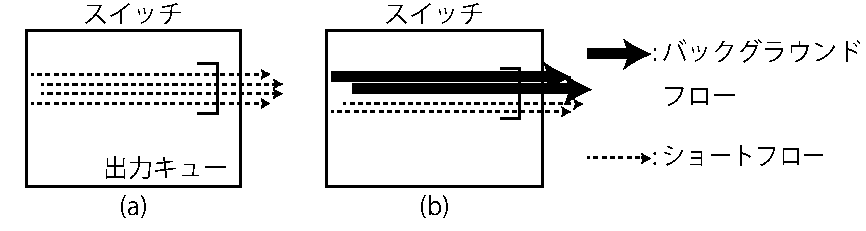
\includegraphics[autoebb, width=170pt]{./img/impairments.pdf}
    \caption{中継スイッチで引き起こすボトルネック}
    \label{fig:impair}
    \end{center}
\end{figure}


\subsubsection{エンドノード - 性能障害}
今日のGbE(Gigabit Ethernet)通信において, 割込み処理は大きなボトルネック要因の一つである.
例えば, 1GbEにおいて64バイトフレームの最大受信可能数は, 毎秒約150万であり, 1パケット受信する度に割り込み処理を行うと,
CPUリソースが枯渇する.
そのため, 割込み処理の回数を抑えることが必要であるが, その分レイテンシが上がる可能性があり, 互いのトレードオフを適切に対処し高い性能を得る必要がある.
また, 今日の多くのCPUはマルチコアであり, CPUリソースを効率的に利用する事が求められている.

{\bf 割込み処理}\\
パケット受信の際のNICによるハードウェア割込みは, 即座に受信処理を行う事ができ, キューイングの遅延を小さくする事ができる.
しかし, 割込み処理が増えれば, その分オーバヘッドが大きくなり, OSの性能が劣化する.
割込み処理を扱う代表的な仕組みとして, ポーリング, interrupt coalescingがある.

ポーリングはNICの割り込みを使わず, タイマーにより定期的にNICの受信キューを監視することで, 割り込み負荷を軽減するソフトウェア技術である.
しかし, NICでパケットを受けてから即座に処理できない為, 遅延が発生する場合がある.
現在のLinuxカーネルにおいては, NAPIにより, 通信量が多く高負荷時にはポーリングが作用する~\cite{NAPI}

interrupt coalescingは, 複数のパケット, あるいは一定期間待ってからをまとめて一度で割り込ませる事で,
割込み回数を減らすハードウェア技術である.
しかし, ポーリングと同様, 即座に処理できない為, 遅延が発生する場合がある.

{\bf プロトコル処理}\\
マルチコア環境においても基本的には一つのNICの受信処理は1つのCPUでしか行えない.
そのため, ハードウェアへのアプローチとして, 1つのNICに複数の受信キューを持たせて, 受信処理をそれぞれのCPUへ分散させている, Receive
Side Scaling(RSS)がある~\cite{RSS}.
しかし, 一般に複数受信キューを持ち, RSS機能があるNICは高価である\cite{intel}.
そのため, 一つしか受信キューを持たないNICであっても, 複数のCPUを分散させるソフトウェア技術として, RPS(Receive Packet
Sterring)がある~\cite{RPS}.
% しかしRPSでは, プロトコル処理とアプリケーション処理のCPUが異なる場合が生じ, その問題を最適化したのがRFS(Receive Flow
% Sterring)がある~\cite{RFS}.
これらの技術により, CPUの複数のコアをより効率良く利用する事ができる.
また, プロトコル処理やアプリケーションでの処理については, RPS等で複数のCPUへと分散させる事ができるが,
その際の割込み処理についてはオーバヘッドが生じる可能性がある.

\section{提案手法}
データセンターにおけるマルチパスネットワークの研究動向と, 並列分散処理アプリケーションが生成する特有のトラフィックパターンが引き起こす機能障害をふまえて,
改善手法を提案する.

提案手法の動機となったのは, MPTCPを用いたデータセンターネットワークモデルである\cite{improving}.
このネットワークモデルでは, エンドノードが複数のNICを持ち, 一つのフローの通信でそれらを同時に利用することでスループットを向上させる.
このような複数経路の効率的利用には, IPベースのルーティングで実現しており, それぞれのエンドノードが持つIPアドレスのペアにより, 通信経路が決定する.
現在のMPTCPの実装では, TCPコネクション確立後に互いのIPアドレスを交換し,
新しいサブフローを形成する仕組みになっているため, サイズの小さいフローの通信では, サブフローを形成するまでに通信が完結する.
以前の我々の解析では, このコネクション確立の際に遅延が生じることが分かっており\cite{mptcp_ana}, どの経路を利用するかによって,
性能性能が大きく変わる.
提案手法の目的は, 低レイテンシなネットワークを実現し,
レイテンシ指向であるショートフローをなるべく遅延を抑えながら通信を完結する事である.
これに対して, NICを追加で設け, 物理的に複数のキューを用意する事で, パケット処理の負荷を分散させる事で実現できると仮定し, その手法として,
複数のNICによるマルチパス環境でのトラフィック制御を提案する.

提案するトラフィック制御では, スイッチ, エンドノードに対してそれぞれのキューの混雑具合を考慮し, 経路を決定する.
本質的な狙いは, フローサイズに従って通信が終えるということであり, 具体的には,
フローサイズの大きいバックグラウンドフローが通信している中でショートフローが発生した場合,
バックグラウンドフローが占有しているキューを避けた経路で通信することでフロー完結時間を抑えるというシナリオを実現するものである.
そのために, 複数経路のうちロングフローレーン(LFL), ショートフローレーン(SFL)を設置し, 優先度によって切り分けて通信を行う.

\subsection{提案手法詳細}
<提案手法ー数式>
\begin{eqnarray}
V_{rs}^G &= -\theta \cdot C_{rs}^G \nonumber \\
V_{rs}^E &= -\theta \cdot C_{rs}^G - \phi
\end{eqnarray}

\subsection{提案手法理論解析}


\section{評価実験}

\section{考察}

\section{結論}

\subsection{今後の課題}

\vspace{1cm}

\clearpage

\begin{thebibliography}{9}
\bibitem{}
参考文献1
\bibitem{}
参考文献2
\end{thebibliography}
\clearpage
\def\thesection{}
\def\thesubsection{\Alph{subsection}}
\setcounter{subsection}{0}
\section{付録}
ここから付録。章番号つけない。代わりにアルファベット。
\end{document}